\section{Aufbau von Ludimus (ES)}
\subsection{Übersicht}
Ludimus selbst ist in zwei Applikationen unterteilt. Eine läuft auf einem Smartphone, welches man als Controller benutzen will.
Dies kann ein Smartphone oder jedes andere Gerät sein, auf welchem Android läuft und wird folglich als Contoller bezeichnet. Die zweite Applikation startet man auf einem Laptop, PC, Tablet oder SmartTV. Diese wird ab sofort als Server bezeichnet. Der User muss auf seinem Controller einen Code eingeben oder scannen, um sich zu der Anwendung, welche auf dem Server läuft, verbindet. Der User bedient nach dem Aufbau der Verbindung die komplette Plattform mit seinem Controller. Die Verbindung ist in der Abbildung \ref{img:Ablauf} nochmal detailliert dargestellt.
\begin{figure}
    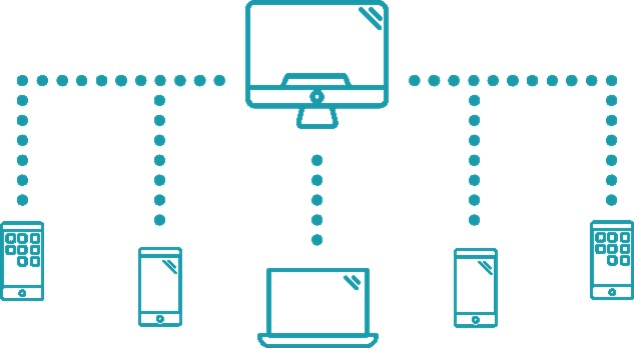
\includegraphics[scale=0.6]{images/ludi.jpg}
    \caption{Aufbau Ludimus}
    \label{img:Aufbau}
\end{figure}
\pagebreak
\subsection{Ablaufdiagram Ludimus}
\begin{figure}
    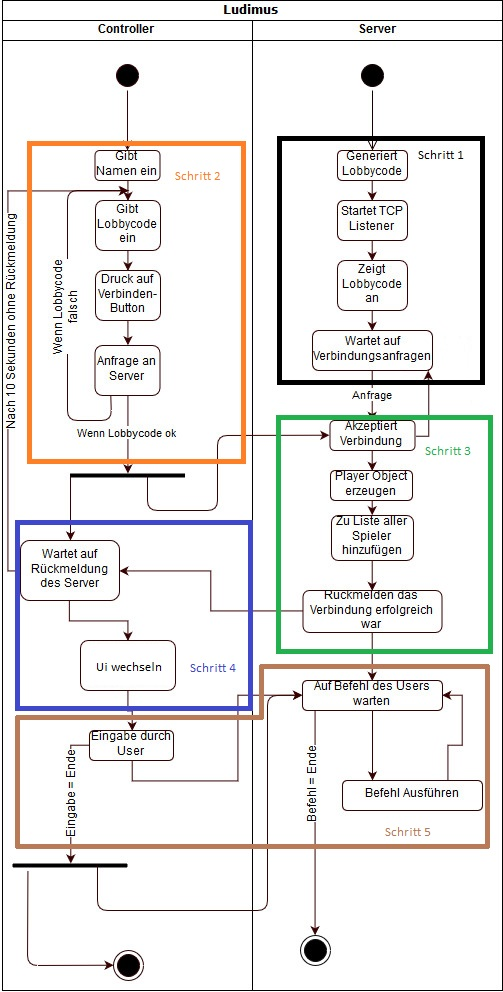
\includegraphics[scale=1.5]{images/Sequence1.jpg}
    \caption{Ablaufdiagram Ludimus}
    \label{img:Ablauf}
\end{figure}
\subsubsection{Erklärung des Ablaufdiagrams(\ref{img:Ablauf})}
\paragraph{Schritt 1}
Im ersten Schritt generiert der Server zunächst einen Lobbycode aufgrund der IP-Adresse des Gerätes.
Genauer ist dies im Kapitel Lobbycodes \ref{lobbycodes} beschrieben. Danach öffnet der Server den TCP Listener, dies sieht im Code so aus:
\newline \textit{ this.listener = new TcpListener(IPAddress.Parse(this.ipAdress), 9393);\newline
this.listener.Start();}\newline
Wichtig ist hierbei, dass der TCPListener nach seiner Instanziierung extra gestartet werden muss. Mehr dazu im Kapitel \ref{tcplistener}. Wenn der TCP Listener erfolgreich gestartet wurde, kann der Lobbycode angezeigt werden, da sich ab diesem Moment Spieler verbinden können. Im Code wird das so realisiert: \newline
\textit{this.LobbyCodeText.text = "Lobbycode: " + this.playermanager.GetLobbyCode();}\newline
Wobei dies in der Initialisierung des UI's und somit in einer anderen Klasse geschieht. Deshalb wird hier auch die
\textit{GetLobbyCode()} Methode des Playermanagers verwendet. \textit{this.LobbyCodeText} ist das TextElement, welches in Unity erzeugt wurde.
Letzter Teil dieses Schrittes besteht darin, den TCP Listener „horchen“ zu lassen, damit er auch auf die Anfragen reagieren kann. Code: \newline
\textit{ var tmpClient = this.listener.AcceptTcpClient();} \newline
Dabei ist jedoch zu beachten, dass this.listener.AcceptTcpClient den Mainthread blockiert und solange wartet, bis eine Verbindungsanfrage kommt. Deshalb wird in Ludimus dies in einem eignem Thread ausgeführt.
\paragraph{Schritt 2}
Bei Schritt 2 gibt der User zunächst seinen Namen und den Lobbycode in Textfelder des UI's ein. Diese sind per 2-Way Binding mit dem Backend verbunden.
Wenn der User nun auf den Verbindungs-Button drückt, wird der Befehl zum Verbinden ausgeführt, dies sieht im Code wie folgt aus: \newline
\textit{this.client = new TcpClient(DecryptLobbyCode(this.lobbycode), 9393);} \newline
Die \textit{DecryptLobbyCode} Methode wird im Kapitel \ref{lobbycodes} genauer erläutert, der TCPClient wurde bereits in Kapitel \ref{tcpclient} behandelt. 9393 definiert den Port, welcher bei Ludimus standardisiert 9393 ist.
\paragraph{Schritt 3}
Der in Schritt 1 bereits beschriebene TCPListener akzeptiert mit \textit{this.listener.AcceptTcpClient();} automatisch eine Verbindung, wenn eine Anfrage kommt.
Wird die Verbindung akzeptiert, wird zunächst ein Player Objekt erzeugt. Im Code: 
\newline 
\textit{var tmpPlayer = new Player(); \newline
tmpPlayer.startPlayer(tmpClient, this, this.internalCounter);}
\newline
Hier wird mit new Player() ein neues Objekt erzeugt, welchem dann mittels der \textit{startPlayer()} Methode alle wichtigen Informationen mitgegeben werden, wie der TCPClient, PlayerManager und Playernumber. In der \textit{startPlayer} Methode wird zusätzlich der Output-Thread geöffnet.
Danach wird das Player Objekt in eine Liste aller Spieler eingefügt, um ständig mit ihm und allen anderen Player Objekten kommunizieren zu können. Am Schluss dieses Schrittes wird dem TCPClient eine Bestätigung geschickt, dass die Verbindung auch wirklich funktioniert hat. Senden von String im Code:
\newline
\textit{
public void SendData(string key, string value)\{\newline
var dat = new byte[4096];\newline
dat = Encoding.ASCII.GetBytes(key + "|" + value + ";");\newline
this.client.GetStream().Write(dat, 0, dat.Length);\newline
this.client.GetStream().Flush();\newline \}
} \newline
Hier wird zunächst ein Byte-Array der Größe 4096 angelegt. In dieses Byte-Array wird dann der String, welchen wir senden wollen, geschrieben. 
Die geschiet mit der \textit{Encoding.ASCII.GetBytes()} Methode in welcher als Parameter der zusendende String steht. 
Der String wird der Methode \textit{SendData} als Key und Value mitgegeben. Mit \textit{this.client.GetStream().Write()} kann man nun auf den Networkstream schreiben.
Wobei man dieser Methode die zu schreibenden Bytes übergibt und angibt, wo angefangen wird zu lesen (da wir vom Anfang lesen wollen 0) und die Länge des zu lesenden Array's übergeben muss.
\paragraph{Schritt 4}
Wenn der TCPClient, also der Controller, nun die Bestätigung bekommt, welchselt er das UI. In dem neuen UI sieht der Spieler den Ludimus-Shop und alle Spiele, welche die ihm zur Verfügung stehen.
Empfangen von Daten im Code: \newline
\textit{ 
var data = new byte[4096];\newline
string responseData = string.Empty;\newline
int bytes = stream.Read(data, 0, data.Length); \newline
responseData = Encoding.ASCII.GetString(data, 0, bytes); \newline}
Wichtig ist dass dies dauerhaft in einem eigenen Thread geschiet, um den MainThread nicht zu blockieren.
Zunächst wird ein neues Byte-Array angelegt, welches 4096 Bytes groß ist. In dieses werden anschließend die gesendeten Daten eingelesen.
Dann muss ein leerer String erzeugt werden, was mit \textit{string.Empty} am saubersten gelöst wird. 
Nun liest man mithilfe von \textit{stream.Read()} in das \textit{data} Array ein. 
Mitgegebn werden dabei das Array, in welches gelesen wird, ein Int, wobei dieser definiert wo im Array angefangen wird einzulesen (in unserem Fall wie bereits erwähnt 0) und die Länge des Arrays in welches gelesen wird.
Mit \textit{Encoding.ASCII.GetString()} wird das Byte-Array zu einem String geparst. 
Dieser String wird in eine Queue gereiht und im MainThread behandelt (siehe \ref{verbindung}). 
Das Lesen von Daten des Network Streams (siehe \ref{ns}) geschieht im Server und Controller gleich.
\paragraph{Schritt 5}
Der letzte Schritt besteht aus dem Warten auf Befehlen am Controller und dem Ausführen von Befehlen am Server.
Es wird zum Beispiel darauf gewartet, dass der User am Controller ein Spiel startet.
Passiert dies, wird mithilfe der in Schritt 3 und 4 beschriebenen Datenübertragung dem Server mitgeteilt, dass er ein Spiel starten soll und dies dann ausführt.
Mehr zu Spielstart unter Kapitel \ref{sec:spielstart}.